\chapter{系统总体方案设计}
\label{chap:system}

\section{开发平台与器件选型}
本系统选用搭载紫光同创 Logos 系列 PGL50H FPGA 的 MES50HP（盘古 50）开发板，
采用紫光同创 PDS 软件完成逻辑设计与实现。平台选型主要考虑视频流处理的并行性、
定点坐标变换的运算需求，以及图像缓存和外部接口的扩展能力。

\subsection{FPGA 芯片及资源配置}
MES50HP 核心板采用的 FPGA 完整型号为 PGL50H-6IFBG484，
属于紫光同创 Logos 系列，采用 40 nm 工艺，速度等级为 $-6$，温度等级为工业级，
封装为 FBG484，共有 484 个引脚。实际 PDS 工程将器件系列、型号、封装和速度等级
分别配置为 Logos、PGL50H、FBG484 和 $-6$，实现记录中的器件标识为
PGL50H-FBG484-6，与板卡手册给出的型号在这些配置项上一致。
根据硬件手册第 2.2.1 节，芯片主要逻辑与存储资源如表~\ref{tab:fpga-resources} 所示\cite{board}。

\begin{table}[htbp]\centering\small
\caption{PGL50H FPGA 主要资源及其在本系统中的用途}
\label{tab:fpga-resources}
\begin{tabularx}{\textwidth}{>{\raggedright\arraybackslash}p{4cm}>{\raggedright\arraybackslash}p{3.5cm}Y}
\toprule
资源类型 & 器件资源总量 & 本系统中的主要用途 \\
\midrule
六输入查找表（LUT6） & 42\,800 个 & 图像预处理、坐标变换及控制逻辑 \\
触发器（FF） & 64\,200 个 & 流水线寄存、状态保持及跨时钟域同步 \\
片内存储块（DRM） & 134 个，每个 18 Kbit & 图像分块缓存、查找表及 FIFO \\
乘法运算单元（APM） & 84 个 & 定点投影变换中的乘法运算 \\
\bottomrule
\end{tabularx}
\end{table}

畸变矫正需要对输出像素逐点计算源图像坐标，并与视频采集、缓存读写和显示输出
协同运行。FPGA 可将上述功能组织为并行模块和多级流水线；其中，APM 为定点乘法
提供专用运算资源，DRM 用于构建局部图像缓存和数据缓冲，LUT 与触发器实现
采样控制、数据调度和接口时序。上述资源配置为本系统的分块逆映射方案提供了硬件基础，
具体资源占用与时序结果在实现验证章节中给出。

\subsection{MES50HP 开发板}
MES50HP 由核心板和扩展底板组成，两者通过高速板对板连接器连接。
核心板集成 FPGA、存储器、配置 Flash、电源及复位电路，构成 FPGA 最小运行系统；
扩展底板提供视频、通信及通用 I/O 接口，便于连接输入输出设备并开展系统联调\cite{board}。
这种结构兼顾了核心处理电路的集成与外围接口的扩展，适合本系统从算法验证到完整
视频链路搭建的开发过程。

核心板提供 50 MHz、27 MHz 单端时钟源及 125 MHz 差分时钟源，其中
50 MHz 用作 FPGA 系统参考时钟，125 MHz 用作 HSST 高速收发器参考时钟。
本工程使用板载 50 MHz 和 27 MHz 参考时钟，并通过 PLL 生成所需的内部工作时钟
和视频输出像素时钟。板卡已有的时钟、电源、复位和 JTAG 配置条件，
为逻辑下载与调试提供了基础。各外部设备的型号、接口电路及连接方式在下一节说明。

\subsection{PDS 开发工具与工程组织}
本系统使用紫光同创 Pango Design Suite（PDS）作为 FPGA 开发工具，
实现工具为 PDS 2025.2 build 211867。PDS 面向紫光同创 FPGA 提供从
HDL 设计输入、逻辑综合、器件映射、布局布线到静态时序分析及位流生成的实现流程，
并配合厂商 IP 完成时钟与存储接口等基础模块的集成。

实际主工程文件为 \path{EmbFPGA.pds}，顶层模块为 \path{hdmi_ddr3_top}。
工程以 Verilog HDL 描述图像处理与控制逻辑，RTL 源码集中在 \path{src/} 目录；
PLL、读写缓存及 DDR3 控制器等 IP 位于 \path{ipcore/} 目录，并通过
\path{.idf} 文件加入工程。引脚、电气属性和时序约束由
\path{src/constraints/hdmi_ddr3_top.fdc} 管理。
开发时依据板卡手册核对引脚及接口电平，在 PDS 中完成综合与布局布线后，
结合资源报告和时序报告检查实现结果，再生成用于板级验证的配置位流。
实现记录关联工具、目标器件、约束文件与配置位流，保证结果可追溯。
\sourcefile{\path{../Pgl50h/EmbFPGA.pds}；\path{../Pgl50h/bitstream/pc_control_20261022_identity.json}}

\section{系统硬件设计}
\subsection{开发板与外部连接}
系统以 MES50HP 开发板为图像处理核心，板载 HDMI 接收、发送与 DDR3 存储接口
构成视频数据通路，UART 接口接收姿态并连接上位机。
图~\ref{fig:mes50hp} 给出开发板及主要接口分布。

\begin{figure}[htbp]\centering
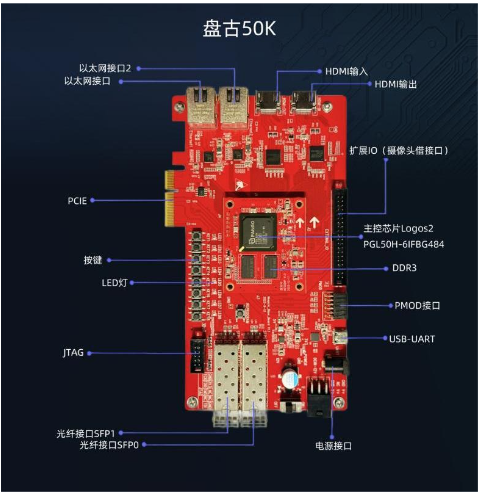
\includegraphics[width=0.66\textwidth]{chapter2/figures/tmp.png}
\caption{MES50HP 开发板及主要接口分布}
\label{fig:mes50hp}
\end{figure}

\subsection{相机与视频输入}
系统使用杰锐微通 USB 工业相机，视频输入规格为 $1920\times1080$、60 fps。
PC 通过 OpenCV 读取原始图像，由独立副屏 HDMI 输出至开发板 HDMI 输入接口；
板载 MS7200 将 HDMI 视频转换为 RGB888 并行像素数据。
该链路便于同时保存原始图像、向 FPGA 供图并开展同源对照分析。
PC 输出显示模式、采集格式和图像尺寸共同决定实际输入条件。

\subsection{视频输出与显示}
FPGA 输出的并行 RGB888 视频由板载 MS7210 编码为 HDMI，
经绿联 USB 采集卡送回 PC，与原始图像并排显示。
显示端独立维持 60 Hz 扫描，新矫正结果在安全帧边界交接。
采集卡与 PC 预览仅承担结果观测，不参与 FPGA 内部的帧率控制。

\subsection{IMU 与姿态输入}
姿态采集使用 RoboMaster C 型开发板，主控为 STM32F407，
传感器为 BMI088 六轴惯性测量单元。
STM32 经 SPI 获取三轴加速度与角速度，以 Mahony 算法解算 yaw、pitch、roll，
量化为有符号 16 bit 数据后，通过 UART 发送至 FPGA。
FPGA 将姿态与源帧关联，在同一帧矫正期间保持参数不变。
姿态采集、坐标约定和通信格式见附录~\ref{app:attitude-estimation}。

\subsection{双轴云台}
相机安装于自研二自由度云台，yaw、pitch 两轴由达妙电机驱动，
用于调整拍摄方向及构造静态、连续转动测试场景。
IMU 与相机保持刚性连接，使姿态输入对应相机的旋转状态。
云台机械轴、传感器轴与图像轴的对应关系决定姿态符号和矫正方向。

\subsection{上位机控制与状态监测}
PC 经板载 CP2102 USB 转串口接口连接 FPGA，
独立控制镜头去畸变、姿态矫正和自适应 Gamma，
并接收功能状态、曲线编号与帧亮度统计。
上位机同时提供双路视频预览、姿态模型显示和图卡质量分析，
软件结构与使用方法见附录~\ref{app:pc-host}。

\section{总体数据通路}
图~\ref{fig:architecture} 给出默认路径。RGB888 输入先完成帧自适应 Gamma，
再转换为 RGB565 以降低帧缓存带宽。采集、渲染和显示并行运行，矫正器使用
源帧对应的姿态和功能快照生成完整结果帧，显示端只在安全的帧边界交接结果。

\begin{figure}[htbp]\centering
\begin{tikzpicture}[
  block/.style={draw=TemplateBlue,rounded corners,fill=TemplateGray,
    align=center,minimum height=1.15cm,text width=4cm,font=\small},
  arrow/.style={-{Latex},thick,draw=TemplateBlue},node distance=0.55cm and 1.3cm]
\node[block] (in) {HDMI 输入 / MS7200\\RGB888};
\node[block,below=of in] (gamma) {帧自适应 Gamma\\RGB888 $\to$ RGB565};
\node[block,below=of gamma] (source) {DDR3 源帧槽 0 / 3\\帧姿态与功能快照};
\node[block,below=of source] (map) {逐像素定点逆投影\\$128\times32$ 双槽分块};
\node[block,right=of map] (sample) {源矩形缓存与采样\\结果块突发写回};
\node[block,right=of source] (result) {DDR3 结果帧槽 1 / 2\\VS 边界交接完整结果};
\node[block,right=of gamma] (out) {RGB565 $\to$ RGB888\\MS7210 / HDMI 60 Hz};
\node[block,right=of in] (ctrl) {IMU UART / CP2102\\姿态、控制与统计遥测};
\draw[arrow] (in)--(gamma);
\draw[arrow] (gamma)--(source);
\draw[arrow] (source)--(map);
\draw[arrow] (map)--(sample);
\node[text=TemplateBlue,inner sep=0pt] at ($(sample.north)!0.5!(result.south)$) {$\uparrow$};
\node[text=TemplateBlue,inner sep=0pt] at ($(result.north)!0.5!(out.south)$) {$\uparrow$};
\draw[arrow,dashed] (ctrl.west)--++(-0.35,0)|- (source.east);
\end{tikzpicture}
\caption{默认配置的系统数据与控制通路}\label{fig:architecture}
\end{figure}

\section{方案选择与实现边界}
\subsection{逆映射与分块访存方案}
正向映射由输入像素寻找输出位置，可能出现输出冲突和未覆盖像素。
本工程采用输出驱动的逆映射，对每个输出像素计算源坐标，再执行采样。
源坐标在外部帧存储中分布不连续，因此使用分块包围矩形与片内缓存，
将多个随机像素访问转换为行内突发读取。

分块仅用于调度和存储，块内仍逐像素计算逆投影，不使用四角网格插值。
输出保持与输入相同的标定内参，不额外裁切或调整焦距；映射超出有效源域时输出黑色。

\subsection{精度、资源与吞吐的取舍}
RGB565 将单像素存储量由 24 bit 降为 16 bit，代价是颜色量化。
默认最近邻采样降低访存和采样开销，但需评估边缘锯齿与高频纹理误差。
透视归一化采用恢复除法流水线，处理吞吐按完整分块通路评价。
最近邻采样、定点精度与颜色量化的影响在图像质量评价中分别考察。

\section{时钟域与帧级工作过程}
系统参考时钟为 50 MHz，视频参考为 27 MHz；视频 PLL 产生 148.5 MHz 输出像素时钟，
DDR 用户接口/渲染域为 100 MHz。输入像素时钟由 HDMI 接收侧提供，
即使同为 148.5 MHz，也应按工程的实际异步关系处理。

帧级过程为：输入 SOF 提交功能设置并锁存姿态，完成源帧采集后允许调度渲染；
渲染期间源槽和结果槽的归属保持不变；最后一个 DDR 写事务完成后登记结果，
显示侧在 VS 边界及相关读事务安全结束后交接。处理未完成时继续显示上一完整结果帧。
\sourcefile{\path{../Pgl50h/src/top/hdmi_ddr3_top.v}；\path{../Pgl50h/src/constraints/hdmi_ddr3_top.fdc}}
